\chapter{Proposal Based Object Detection and Classification}

In this section the theoretical overview of the logo retrieval system will be presented. First of all the fully convolutional networks will be introduced in section \ref{s:c-fullyconvnet}. Section \ref{s:c-rpn} explains region proposal systems for generating candidate object locations on an image. Afterwards, the section \ref{s:c-rcnn} describes region based convolutional neural networks for object detection and classification. The improvement of this method, the fast region based convolutional neural networks will be detailed in the section \ref{s:c-fastrcnn}. Folowing this, the further development, the faster region based convolutional neural networks will be reviewed in the section \ref{s:c-fasterrcnn}.

\section{Fully Convolutional Neural Networks}\label{s:c-fullyconvnet}
A neural network is fully convolutional, if it does not contain any fully connected layers. Firstly Matan et.al. used FCNs for recognizing strings of digits. Long et. al. proposed \cite{DBLP:journals/corr/LongSD14} how to transform a deep neural network with fully connected classifier layers at the end, to a fully convolutional network. For this purpose the fully connected layers at the end of the network are to be converted to convolutional layers.
\smallbreak
Since the number of weights of a neuron in a fully connected layer is defined by the shape of the data of the layer, the trained network can process only a fix-sized input. As a fully convolutional network does not have fully connected layer anymore, it has the advantage of being able to train and test with images of arbitrary sizes.
\smallbreak
The outputs of such a network are two dimensional feature maps, which can be used as heatmaps per class. These convolutional maps can also be used directly for semantic segmentation, where each pixel of an image should be classified.
Nowadays fully convolutional networks are essential part of state-of-the-art object detectors, yielding better performance, image size agnosticism, as well as shorter training and inference times.

\section{Region proposal systems}\label{s:c-rpn}
To recognize different objects on an image, like logos, small regions should be considered. The easiest way to search for these locations is the exhaustive sliding window search, applied on multiple scales. Although, as section \ref{s:c-objectdetection} presents, this induces a lot of computational costs. In order to reduce this computational burden, region proposal systems can be utilized. Region proposals are possible object locations on an image.
\smallbreak
Earlier computer vision solutions used external proposal systems. This means that the proposals of every image should be pre-calculated before training or inference. One of the most popular region proposal methods is selective search \cite{Uijlings13}. It merges neighbor regions according to a similarity score in a bottom-up fashion. It processes an image under 2s on the CPU, which precludes the possibility of real time applications. Edge Boxes \cite{edge-boxes-locating-object-proposals-from-edges} are efficiently calculating the number of contours in a box, and ranking them according to that almost real time. Today, as section \ref{s:c-fasterrcnn} introduces, the proposal system is already part of the neural network.

\section{Region Based Convolutional Neural Networks}\label{s:c-rcnn}

This section gives a brief overview about how faster region based convolutional neural networks evolved.

\subsection{Regions with Convolutional Neural Network Features}
Although this network is already historical, it is worth to mention it, because it helps to understand the improvements of the later systems. Region based convolutional neural networks \cite{DBLP:journals/corr/GirshickDDM13} consist of four separate systems. Firstly, region proposals are generated external with selective search. There will be altogether 2000 object positions considered. Secondly, each region of the possible object locations is warped to a size of 227x227, and then the feature vector of every single region is extracted with a CNN. The network is pretrained on the ImageNet dataset \cite{NIPS2012_4824}, and then fine-tuned on the final classes. The network is run on every region proposal bounding boxes, to extract vectors with a fixed-size. These vectors will to be written to the disk. Thirdly, a set of class-specific linear SVM is used to classify the specific region. At last bounding box regressions is run, to reduce the mislocalization of the object. This happens outside of the network.
\begin{figure}[h!]
	\centering
	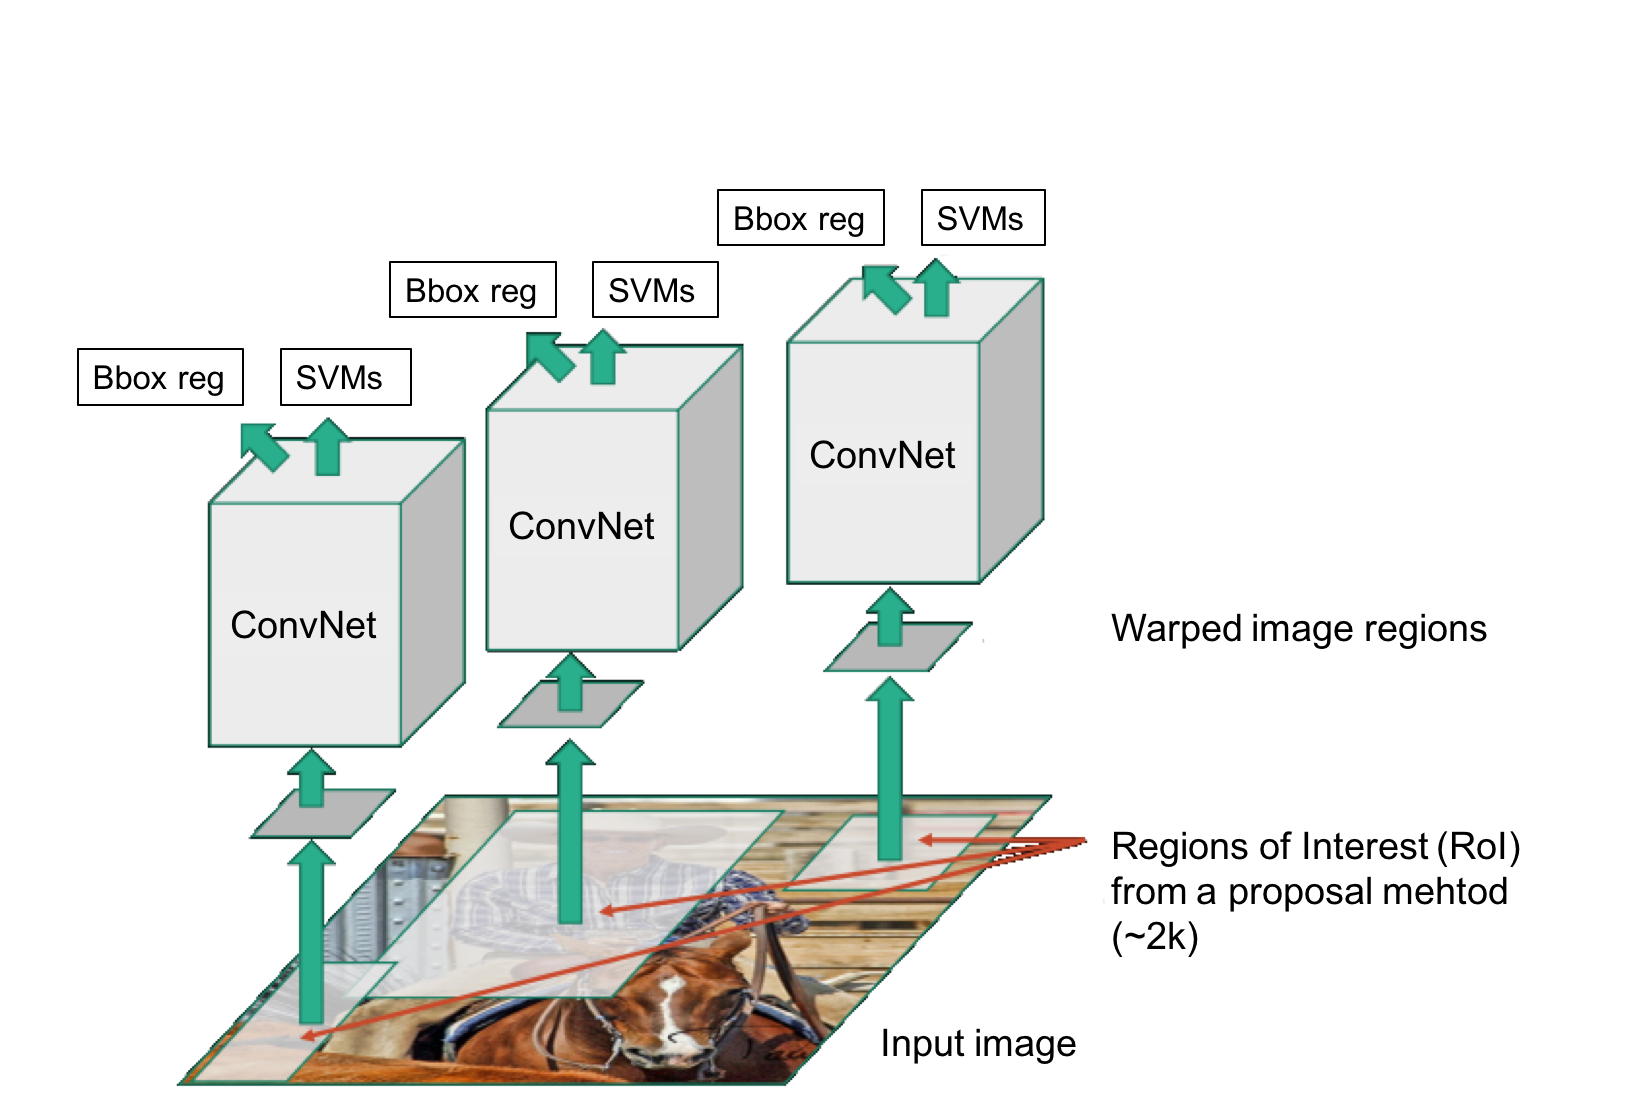
\includegraphics[width=12cm]{images/mt/rcnn.png}
	\caption{R-CNN takes external region proposals, warps the region to a uniform shape, and extracts the features separately. The extracted features are then used to classify the region, and calculate bounding box regression externally.}
	\label{fig:rcnn}
\end{figure}

\subsection{Fast Region Based Convolutional Neural Network}\label{s:c-fastrcnn}
Fast Region based CNNs \cite{Girshick:2016:RCN:2881668.2882239} are aimed to improve the classification accuracy and feature vector extraction speed of the interest regions, generated also with selective search. An intermediate convolutional feature map is extracted from the whole input image with a fully convolutional neural network, also called as base network in \citep{journals/corr/SermanetEZMFL13}. The output is a downscaled feature map, which is fed to the so called RoI (region of interest) pooling layer. This layer crops regions from the map according to the appropriate downscaled region proposals, and executes a modified version of max pooling on each regions, which results in a convolutional map with a fixed-shape, regardless the size of the region.

After the pooling, fully connected layers are used to calculate the final class probabilities and bounding box regressions for each region. The output of the bounding box regression are class specific small position and size adjustments, needed to refine the rough object locations.
\smallbreak
The improvements of this method compared to the previous region based CNN introduced in section \ref{s:c-rcnn} are as follows:
\begin{itemize}
	\item\textbf{Joint feature extraction:} much shorter training and inference time is achieved by the lower computational redundancy of running convolutional layers on the whole image only once, rather then for every proposed regions.
	\item\textbf{One network:} the feature extraction and the classification happens in the same network. This has more advantages:
	\begin{itemize}
	        \item This results again in faster test and training times, due to the unnecessity of writing the extracted feature vectors to disk, which incidentally could require hundreds of gigabytes of storage \cite{Girshick:2016:RCN:2881668.2882239} for the VOC07 trainval set \cite{pascal-voc-2007}.
	        \item As the backpropagation is implemented through the RoI pooling layer, the whole network, together with the convolutional layers, can be trained jointly, against earlier implementations, like R-CNN \cite{DBLP:journals/corr/GirshickDDM13} or spatial pyramid pooling networks (SPPnet) \cite{DBLP:journals/corr/HeZR014}.
	\end{itemize}
	\item\textbf{Minibatch from a few images:} Faster training speed is achieved by collecting a minibatch only from two images, rather than every region from different images. This method is proved to converging within similar times, despite the high correlated regions.
\end{itemize}
The network is trained with a multi-task loss function for classification and bounding box regression, defined as:
\begin{equation}\label{eq:c-frcnn-loss}
	L(p, u, t^u, v) = L_{cls}(p, u) + \lambda [u \ge 1] L_{loc}(t^u, v)
\end{equation}
where $p$ is the computed class probabilities, $u$ is the groundtruth class, $t^u$ is the predicted bounding box offsets for every classes, and v is the groundtruth bounding box position and size.
Since the probabilities are calculated with softmax as usual, the log loss is used for the classification error: $L_{cls}(p,u) = -logp_u$. For bounding box regression loss, a smooth version of L1 loss is used, which is defined as follows:
\begin{align}\label{eq:c-smoothl1loss}
	L_{loc}(t^u, v) = \sum\limits_{i \in (x, y, w, h)} smooth_{L_{1}} (t_{i}^u, v_i)\\
	smooth_{L_{1}} (x) = \begin{cases}
               0.5 x^2 & \text{if } \abs{x} < 1\\
               \abs{x}-0.5 & \text{otherwise}
            \end{cases}
\end{align}
 is As the background class has the 

The network is trained for K+1 classes, where K is the number of object classes, and the background is also modelled as a separate class. During training, the positive examples are chosen, regarding the intersection over union (IoU) value to the groundtruth. This value is widely used for measuring the overlapping between regions, regardless the actual size of the regions. The calculation between two regions, $R_1$ and $R_2$ is as follows:
\begin{equation}\label{eq:c-iou}
        \frac{area ( R_1 \cap R_2 )}{area ( R_1 \cup R_2 )}
\end{equation}
For positive training examples there are thoose regions applied, which have an IoU with the groundtruth at least 0.5. For the background class are the examples with IoU [0.1,0.5) used.
\begin{figure}[h!]
	\centering
	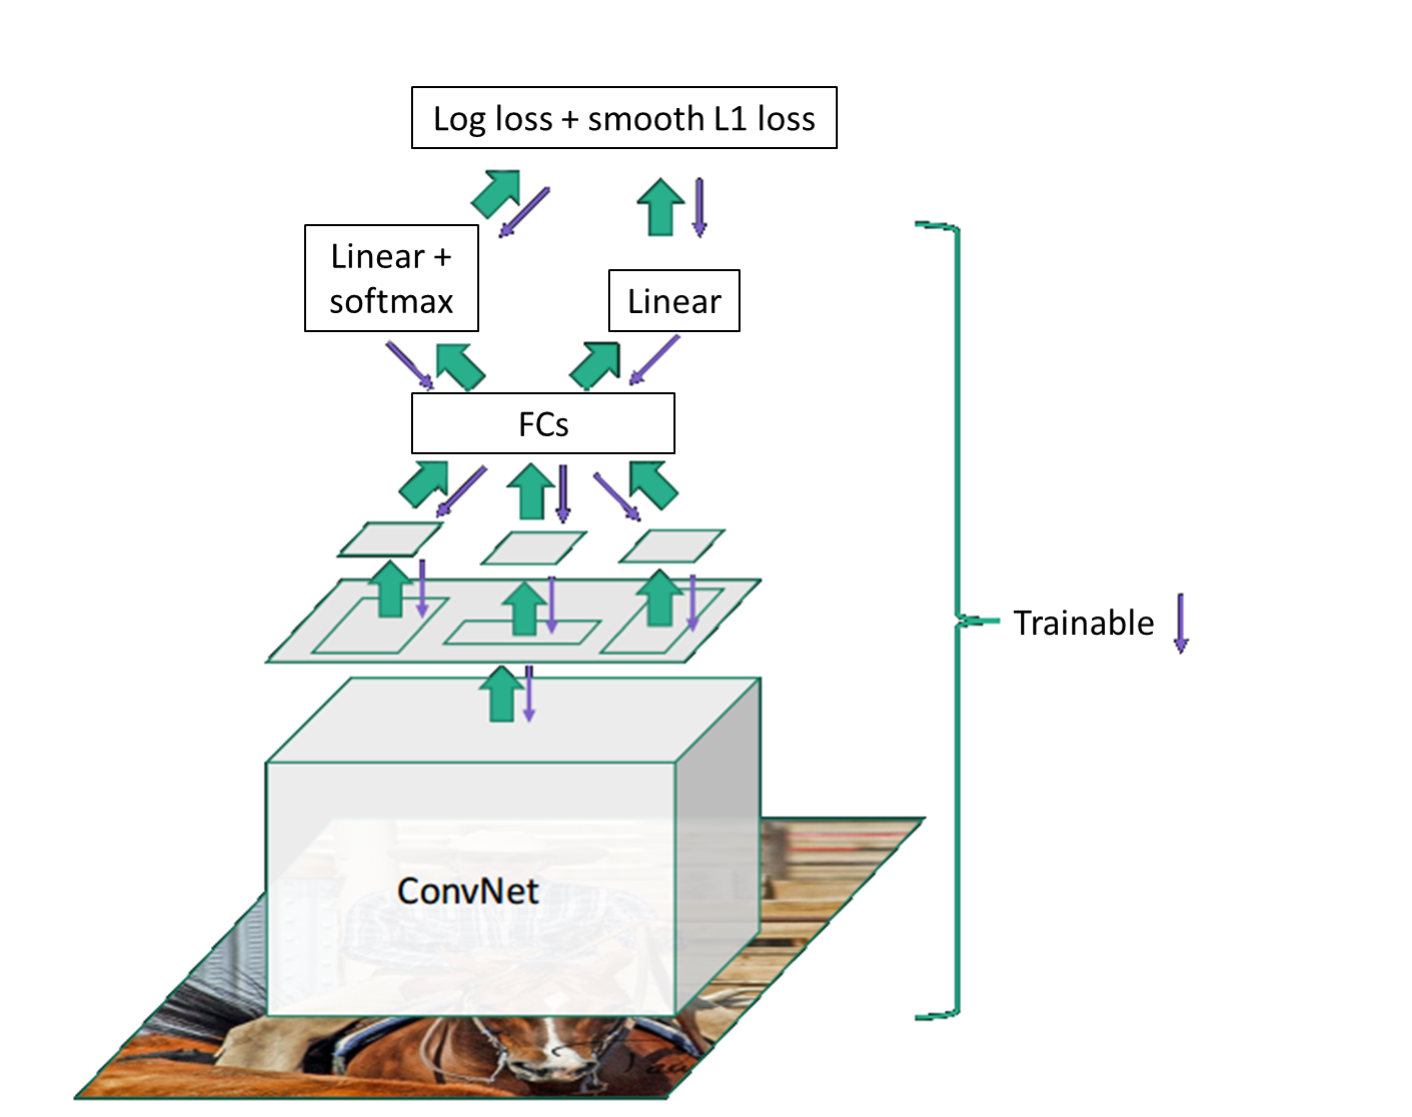
\includegraphics[width=12cm]{images/mt/fast-rcnn.png}
	\caption{Fast R-CNN uses external proposals, then infers the complete image with a fully convolutional network. The proposals is then used to crop regions from the feature map with RoI pooling. The cropped region is then classified and the region coordinates are adjusted with a fully connected network.}
	\label{fig:rcnn}
\end{figure}

\subsection{Faster Region Based Convolutional Neural Network}\label{s:c-fasterrcnn}

A great disadvantage of the Fast R-CNN method is, that the region proposals are generated externally. Girshick et.at. introduces Faster R-CNN \cite{NIPS2015_5638}, which generates the interest regions within the neural network nearly cost-free (10ms pro image). This system consists of a region proposal system and a Fast R-CNN object detector.

\subsubsection{Region Proposal Network}

The convolutional feature map, extracted by the base network, is processed by the RoI pooling layer. Additionally a thin fully convolutional network, the region proposal network (RPN), is also utilized on the convolutional maps, to generate the proposals. Reference boxes, called "anchors" are generated at every position of the conv feature map, in different scales and different aspect ratios. This ensures the scale invariance of the objects. A convolutional layer with 3x3 kernel extracts a fixed-size vector from every window of the conv map, where in each window 9 anchors are considered. As the fully convolutional network iterates through the conv map in a sliding window fashion, translation invariance is granted. An objectness score and bounding box offset is then calculated for every anchor, by different classifiers and regressors, specialized in a specific scale and aspect ratio.
\begin{figure}[h!]
	\centering
	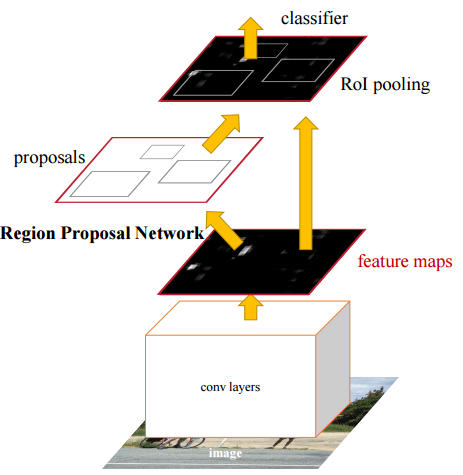
\includegraphics[width=8cm]{images/mt/faster-rcnn.png}
	\caption{Faster R-CNN consists of a Fast R-CNN and a region proposal network (RPN). Fast R-CNN is responsible for the feature map extraction from the whole image, and classify regions from that. The RPN is an in-network implemented proposal system, for generating candidate object locations in a fast way.}
	\label{fig:faster-rcnn}
\end{figure}
\subsubsection{Training}
As the RPN is a class agnostic object detector, it should detect all the types of objects, which the network is trained on. For this purpose, the class informations, during training of RPN, can be discarded. Positive examples are collected from the proposals with an IoU higher than 0.7 with any groundtruth. Negative label is assigned for regions, which have an IoU, lower than 0.3.

Since the objective of the RPN is the same as for Fast R-CNN, namely to classify regions and regress bounding box coordinates, the loss functions for training the RPN can the same multi-task loss, which are used for training a Fast R-CNN, detailed in section \ref{s:c-fastrcnn}.

Earlier versions of the system suggested to train the complete system in an alternating way. First the RPN will be trained with a CNN, pretrained on e.g. the ImageNet dataset. The trained RPN will then be used to propose regions, and train the Fast R-CNN part with them. The CNN of the fine-tuned Fast R-CNN is then used to train the RPN again, and this process is repeated iteratively. Later, it has been proven, that training the whole network of the faster R-CNN can be performed in an end to end manner, with marginal performance drop. This means, that all the parts of the system can be trained jointly.